\documentclass[12pt]{article}
\usepackage{hyperref}
\usepackage{natbib}
\usepackage{amsmath}
\usepackage{nicefrac}
\usepackage[usenames,dvipsnames]{xcolor}
\usepackage{graphicx}
\usepackage{footnote}
\usepackage{rotating}
%\usepackage{slashbox}
\usepackage{afterpage}
\usepackage{float}
\usepackage{color}
\usepackage{array}

\usepackage[margin = 1.0 in]{geometry}
\usepackage{natbib}

\renewcommand{\bottomfraction}{.9}
\renewcommand{\topfraction}{.9}
\renewcommand{\textfraction}{0.1}
\renewcommand{\floatpagefraction}{.9}


%%%%%%%%%%%%%%%%%%%%%%%%%%%%%%%%%%%%%%%%%%%%%%%%%%%%%%%%%%%%%%%%%%%%%%%%%%%%
%   document style macros
%%%%%%%%%%%%%%%%%%%%%%%%%%%%%%%%%%%%%%%%%%%%%%%%%%%%%%%%%%%%%%%%%%%%%%%%%%%%
\def\gtrsim{\mathrel{\hbox{\rlap{\hbox{\lower4pt\hbox{$\sim$}}}\hbox{$>$}}}}
\def\lessim{\mathrel{\hbox{\rlap{\hbox{\lower4pt\hbox{$\sim$}}}\hbox{$<$}}}}
\newcommand{\ddg}{$\Delta\Delta G~$}
%%%%%%%%%%%%%%%%%%%%%%%%%%%%%%%%%%%%%%%%%%%%%%%%%%%%%%%%%%%%%%%%%%%%%%%%%%%%

\graphicspath{{../figures/}}

\title{Variation in site entropy explains differences in structure-sequence relationships of proteins}
\author{Eleisha L. Jackson$^{2^*}$, Amir Shahmoradi$^{1*}$, Claus O. Wilke$^{2^{**}}$}
\begin{document}

\date{\today}
\maketitle


\noindent
$^1$ Department of Physics, The University of Texas at Austin, Austin, TX 78712, USA \\
$^2$ Institute of Cellular and Molecular Biology, Center for Computational Biology and Bioinformatics, and Department of Integrative Biology, The University of Texas at Austin, Austin, Texas, 78712 USA\\

\noindent $^{*}$These authors contributed equally. \\

\bigskip
\noindent
$^{**}$Corresponding author\\
%$\phantom{^*}$Email: amir@physics.utexas.edu\\
$\phantom{^{** }}$Email: wilke@austin.utexas.edu\\
%$\phantom{^*}$Phone:{ \color{red} Need a phone} \\
$\phantom{^{**}}$Phone: +1 512 232 2459\\

\bigskip
\noindent
Manuscript type: research article\\
\bigskip
\noindent  Keywords: protein evolution, relative solvent accessibility, site variability


\begin{abstract}
{\color{red}Recent work has shown that structural properties are capable of predicting site-specific sequence variability for a given protein. However, the strength and significance of these structure-sequence relations appear to vary widely among different proteins, with absolute correlation strengths ranging from $0.1$ to $0.8$. }
\end{abstract}
\vfill
\vfill
\def\thefootnote{\fnsymbol{footnote}}
\setcounter{footnote}{0}


\section{Introduction}
\label{sec:intro}

Proteins are subject to a number of biophysical and functional constraints \citep{Scherreretal2012, Wilkeetal2010}. These constraints result site-specific patterns of sequence variability within a protein. Recently several site-specific structural properties that can explain patterns of sequence variability in proteins have been identified. One of the earliest examples is Relative Site Accessibility (RSA). \cite{Fransozaetal2009} identified RSA as the strong predictor of evolutionary rate and found that residues that are buried in the core of proteins tend to be more conserved than exposed residues close to the surface of the protein. In their analysis they considered the ability of both RSA and various definitions of residue packing density to predict evolutionary rate. They found that RSA and evolutionary rate shared a significant linear relationship. Afterwards, several other works \citep{Ramseyetal2011, Scherreretal2012} also found that RSA as a very significant predictor of evolutionary rate and found this linear relationship as well. However, these papers all have the same flaw. During the course of their analysis they binned the protein sites and average over all sites within a bin when looking at the trend of RSA. This process may have produce artifacts that account for this strong linear trend. \\
\indent Recently, \cite{Yehetal2014} performed a similar analysis on a series of enzyme monomer proteins and found that packing density, as defined by CN and WCN \citep{Liaoetal2005, Yehetal2014, Huangetal2014}, was the strongest determinant of site variability.  A year later, \cite{Shahmoradietal2014} also performed a site-wise analysis on a series of viral proteins. In this analysis they found that RSA had the strongest correlation with site variability as opposed to local packing density. Additionally the effect seen between CN and WCN was of a much smaller magnitude as compared to \citep{Yehetal2014}. Therefore the relationship between local pacing density, RSA and site-specific measures of sequence variability is not well understood. Here we attempt to reconcile the work done in this area. We find that site variability is the primary determinant of the strength of structure-sequence relationships and some differences in previous work can be explained in terms of differing levels of site variability. \\

\section{Materials and Methods}
\label{sec:mam}

    \subsection*{Structures, sequences, and measures of sequence properties } 
    The results presented in this work are based on two datasets. The first is a dataset of $209$ monomeric enzymes taken from \cite{Huangetal2014}, originally from \cite{Yehetal2014}.The original dataset was comprised of $213$ proteins but we removed four of the proteins (PDB IDS: 1BBS, 1BS0, 1DIN, 2HPL) that had did not have data at insertion sites. Briefly, these proteins are all enzyme monomers   randomly picked from the Catalytic Site Atlas $2.2.11$ \citep{Porteretal2004} with protein sizes in the sample ranging from $95$ to $1287$ residues in length. For each structure we had a corresponding alignment of up to 300 homologous sequences.  The second dataset was taken from \cite{Shahmoradietal2014} and is comprised of nine viral proteins. The viral proteins range from 122 - 557 residues in length and each structure is accompanied by a sequence alignment of up to 2362 homologous sequences. Sequence alignments for both datasets were constructed by aligning the amino-acid sequences using the alignment software MAFFT \citep{Katohetal2002, Katohetal2005}, specifying the auto flag to select the optimal algorithm for the given data set. The alignments were then used to calculate the site-specific measures of sequence variability for each individual protein in both datasets. To do so, we relied on two independent methods of measuring sequence variability. First, we calculated the Shannon entropy ($H_i$) -- the sequence entropy at each alignment column $i$:
    \begin{equation}
        \label{eqn:shannon}
        H_i = -\sum_j P_{ij}\ln P_{ij}
    \end{equation}

    where $P_{ij}$ is the relative frequency of amino acid $j$ at position $i$ in the alignment. The sequence entropy is a measure of variability at each site. We also calculated a measure of site-specific evolutionary rate for each protein using software Rate4site. First the Maximum Likelihood phylogenetic trees were inferred with RAxML, using the LG substitution matrix and the CAT model of rate heterogeneity \citep{Stamatakis2006, Stamatakis2014}. For each structure, we then used the respective sequence alignment and phylogenetic tree to infer site-specific substitution rates with Rate4Site using the empirical Bayesian method and the JTT model of sequence evolution \citep{Mayroseetal2004}.

    \subsection*{Calculation of Structural Properties}
In our analysis we used two types of measures of local packing density used in previous studies: Contact Numbe r(CN) and Weighted Contact Number(WCN). For the purposes of our comparison between the two datasets of interest we used the CN and WCN for the enzyme proteins calculated in \cite{Huangetal2014} and the CN and WCN values for the viral proteins from \cite{Shahmoradietal2014}. In both of these works and in \cite{Yehetal2014}, WCN and CN are both defined the same.  Contact Number is defined as the number of $C_{\alpha}$ within a pre-redefined radius, $r_0$. In this case, $r_0$ = 13 as in the previous papers. Weighed Contact Number for a residue, $i$, is defined as in (Liao et al 2005, Huang et al 2014), as:
	
	\begin{equation} \label{wcn_eqn}
		\text{WCN}_i = \sum_{i \neq j}^{N} \frac{1}{r_{ij}^2 } 
	\end{equation}
	
	where $r_j$ is the length between the $C_{\alpha}$ of residue $i$ and residue $j$ in a protein of length $N$ \citep{Yehetal2014}. 

\indent We used DSSP \citep{Kabschetal2005} to calculate the Accessible Surface Area (ASA) for each site. We then normalized the ASA for each site by the theoretical maximum solvent accessibility values of \cite{Tienetal2013} to obtain the Relative Solvent Accessibility (RSA) for all individual sites in all proteins. \\

All data and analysis scripts required to reproduce the work are publicly available to view and download at \url{https://github.com/wilkelab/rate_variability_variation}.

\section{Results}
\label{sec:results}

We calculate the strength between the structural properties and site variability by calculating the Spearman correlation, $\rho$,  between the structural property (solvent exposure and local packing density) and site variability, as measured by either evolutionary rate or site entropy. On average the correlations between CN and entropy are larger in absolute magnitude in the enzyme proteins as compared to viral proteins. The average $\rho$ between each structural property and each measure of site variability (entropy and evolutionary rates) can be seen in {\color{red}Table 1 and Table 2}. The viral proteins experience much lower site variability. Figure 1 shows the correlations between CN and entropy for the virus and enzyme proteins. Even though on average the correlations in the enzyme proteins are larger as reported, by \cite{Yehetal2014}, the virus proteins still have correlation strengths that are comparable to some of the enzyme proteins with lower correlations. 

\indent  The average site variability of a given protein does not seem to be a significant determinant of the strength of structural correlations (Figure 1A, 2A, 3A). However, when examining the variance of entropy there is a clear trend within the enzyme proteins.  Proteins with a higher variance in site variability across the protein typically have have lower correlations (Figure 1B, 2B, 3B). If you extrapolate the trend from the enzyme proteins, the viral proteins follow a similar trend. The correlation between the $\rho$ between RSA and entropy and the variance of entropy is positive. The correlation is negative between local packing density (both WCN and CN) and the variance of entropy is negative. Unlike with entropy, there is no relationship between variance of evolutionary rates at sites and any of the measured structural properties. There also is a wide spread int he variance of the evolutionary rates across proteins for both the enzyme and viral proteins. 


\section{Discussion}
\label{sec:dcr}
{\color{red}SOME DISCUSSION.....} \\

Need a section about:
Rate4Site is completely different from the entropy variation and we do not know why. Explain the difference. 

\section{Acknowledgements}
The authors acknowledge the Texas Advanced Computing Center (TACC) at The University of Texas at Austin for providing High-performance computing resources. ELJ is is funded by a National Science Graduate Research Fellowship, grant number DGE-1110007. COW is funded by {\color{red} Which grants??}.  AS is funded by {\color{red} Which grants??}.
....

%\clearpage
%\newpage

%\cleardoublepage

\bibliographystyle{peerj} %"style
\bibliography{manuscript_bib} %expected file "my refs.bib"

\cleardoublepage
\section*{Figures}

    \begin{figure}[H]
            \centerline{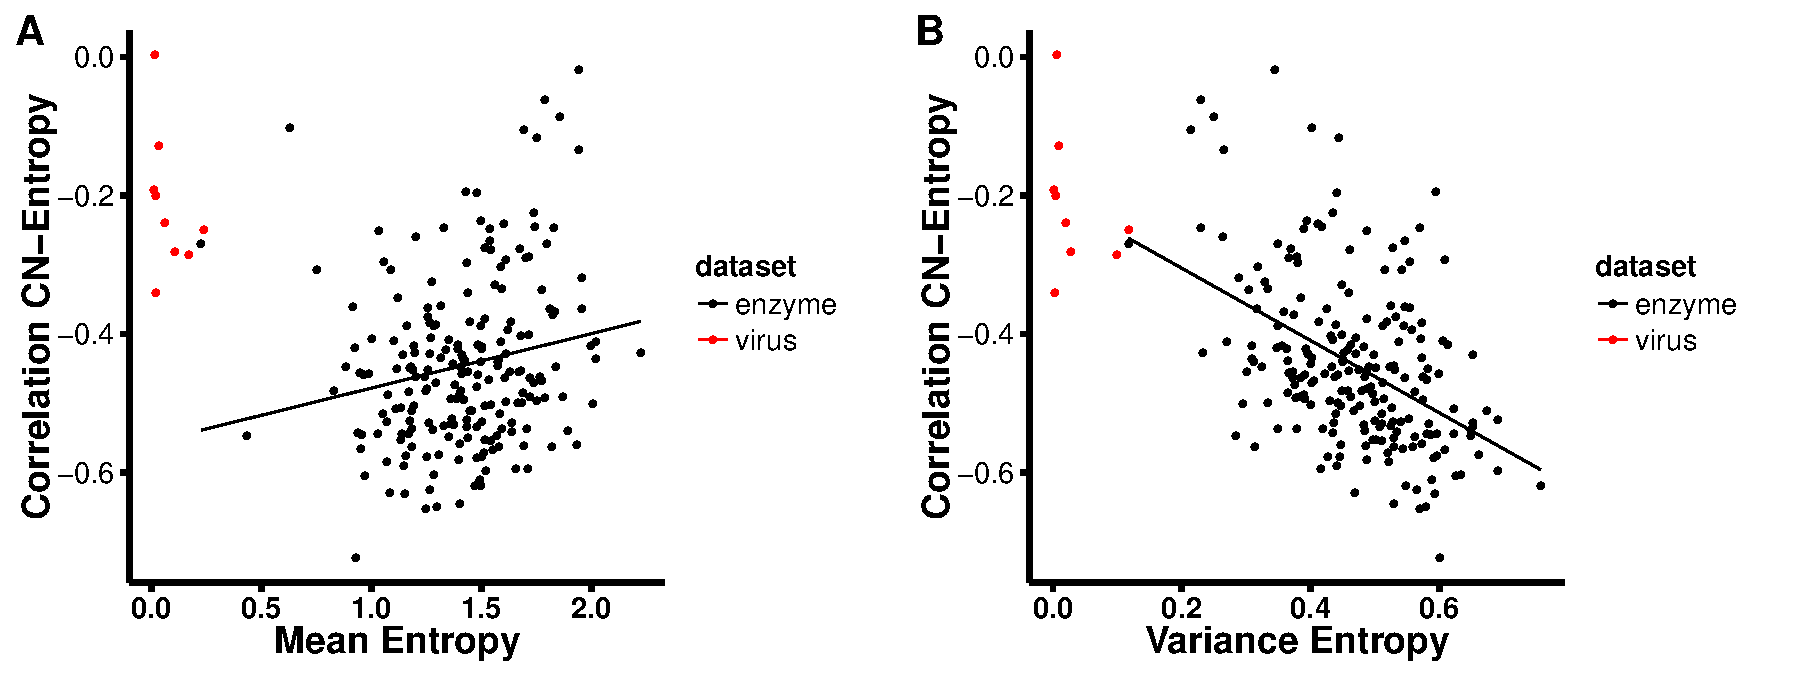
\includegraphics[width=7.5in]{entropy_cn_cor.pdf}}     
            \caption{NEED A CAPTION!!!.}
            \label{fig:seqent_structure_cors}
    \end{figure}


    \begin{figure}[H]
            \centerline{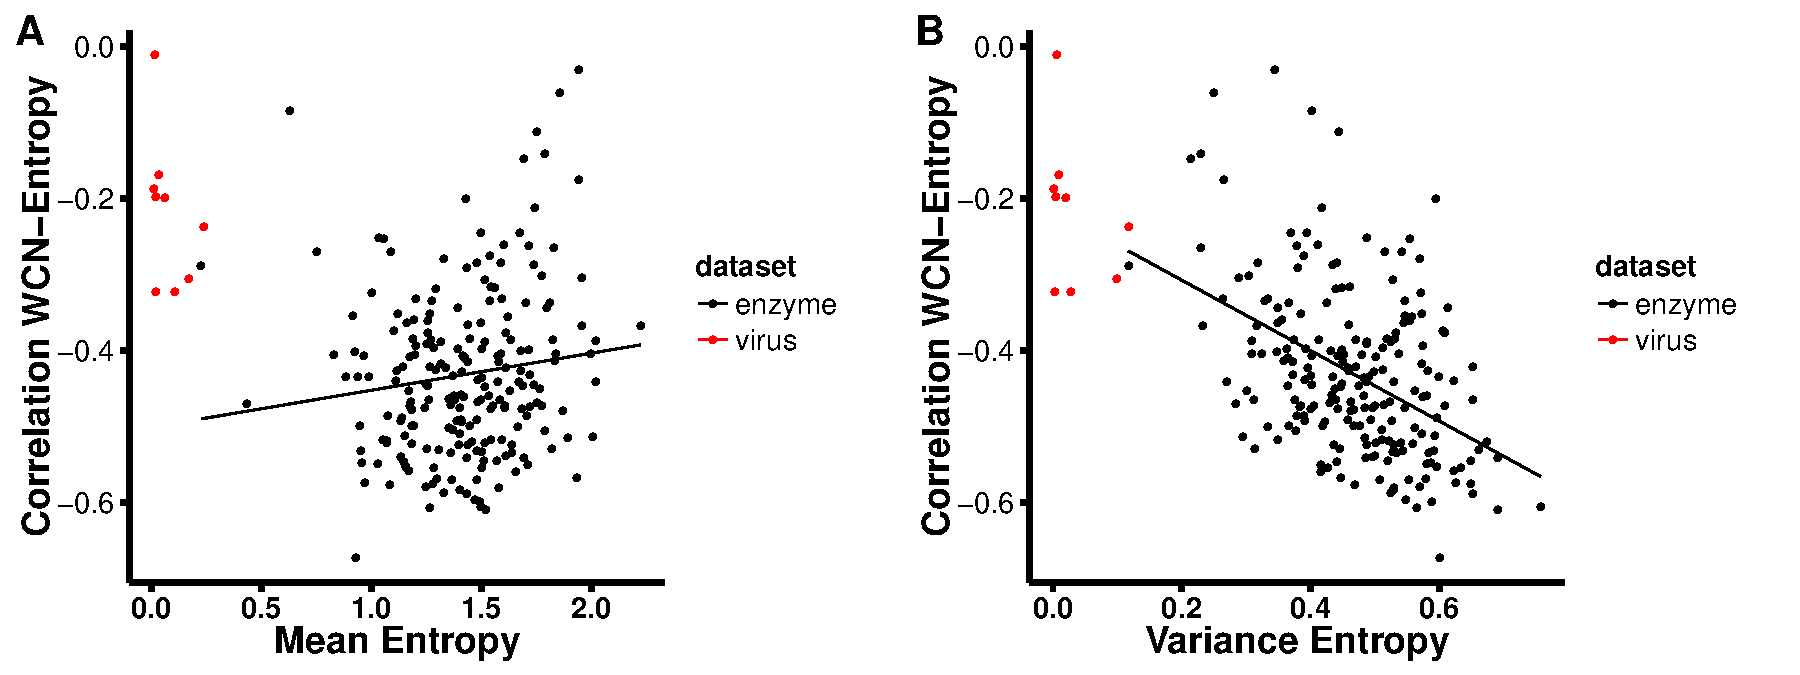
\includegraphics[width=7.5in]{entropy_wcn_cor.pdf}}     
            \caption{NEED A CAPTION!!!.}
            \label{fig:seqent_structure_cors}
    \end{figure}


    \begin{figure}[H]
            \centerline{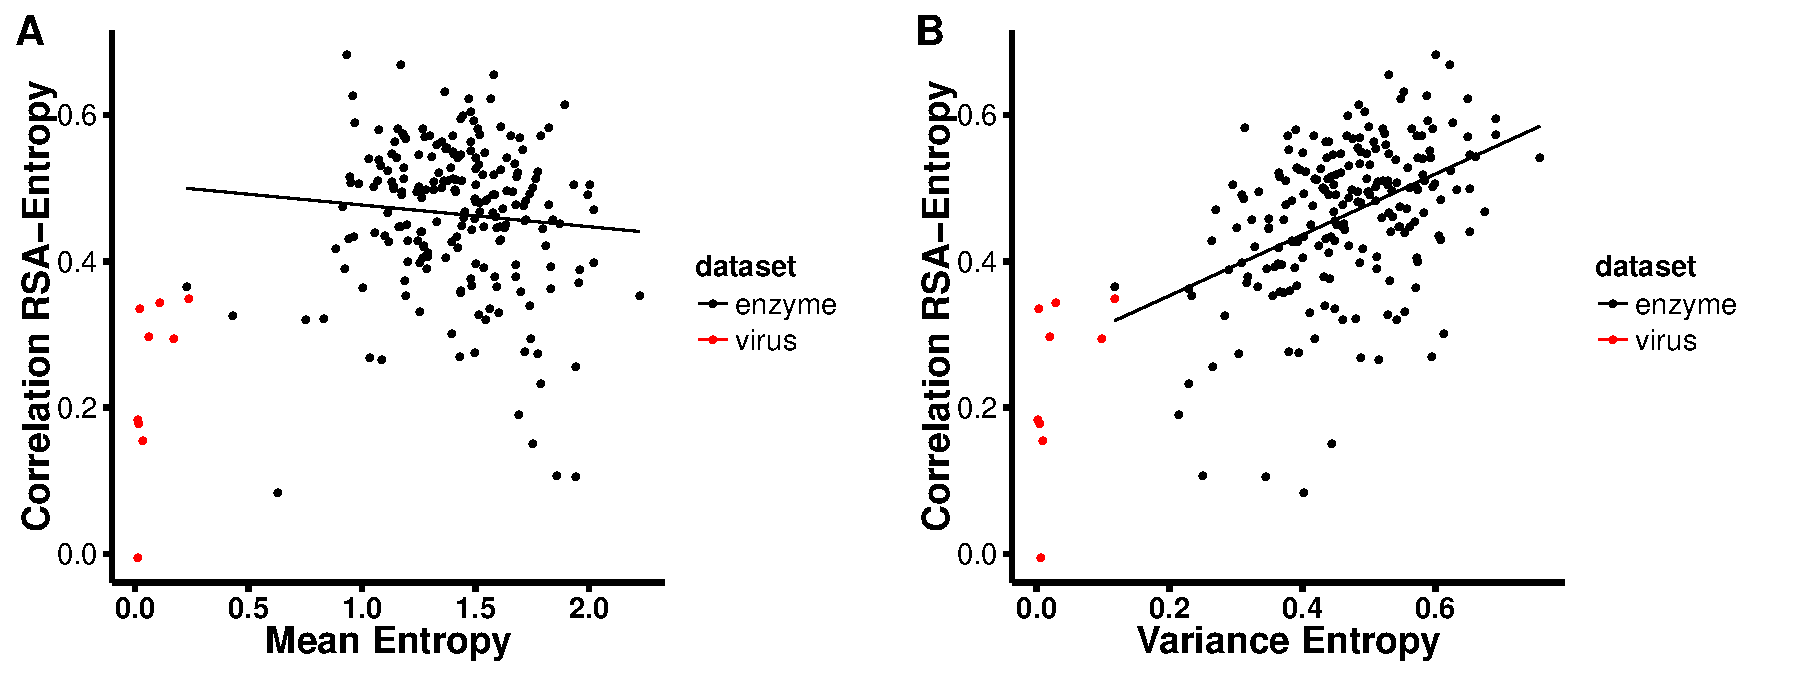
\includegraphics[width=7.5in]{entropy_rsa_cor.pdf}}     
            \caption{NEED A CAPTION!!!.}
            \label{fig:seqent_structure_cors}
    \end{figure}
  
       
        \begin{figure}[H]
            \centerline{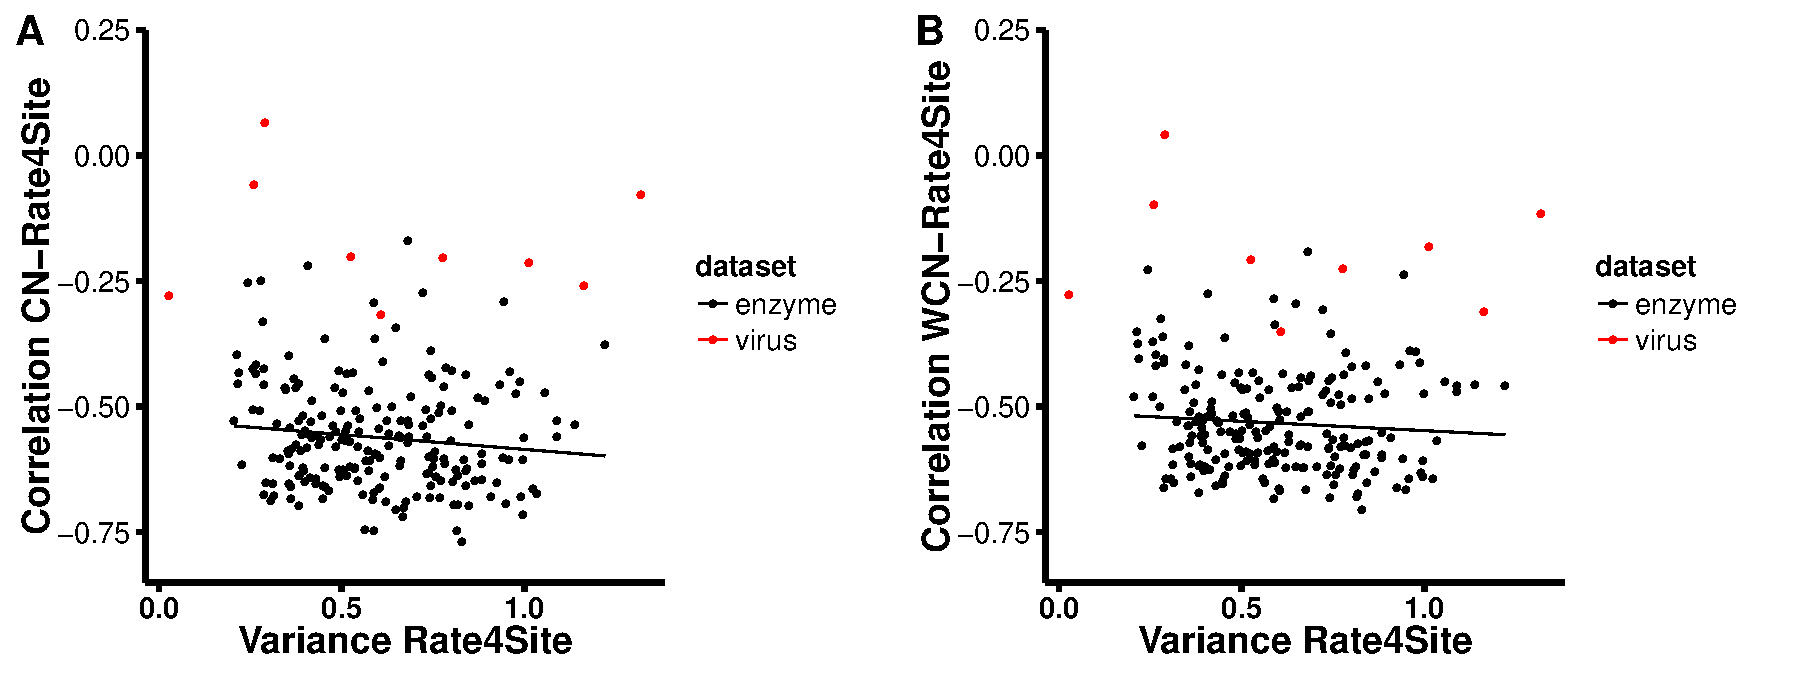
\includegraphics[width=7.5in]{rate_cor.pdf}}     
            \caption{NEED A CAPTION!!!.}
            \label{fig:seqent_structure_cors}
    \end{figure}
        
            \begin{figure}[H]
            \centerline{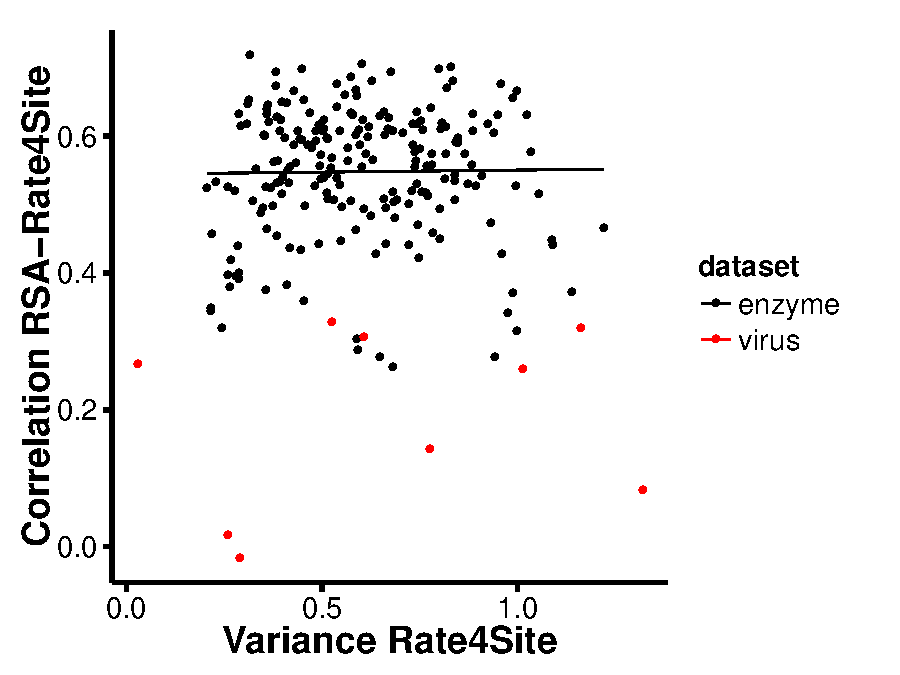
\includegraphics[width=5.0in]{var_rate_rsa_cor.pdf}}     
            \caption{NEED A CAPTION!!!.}
            \label{fig:seqent_structure_cors}
    \end{figure}
    
        \begin{figure}[H]
            \centerline{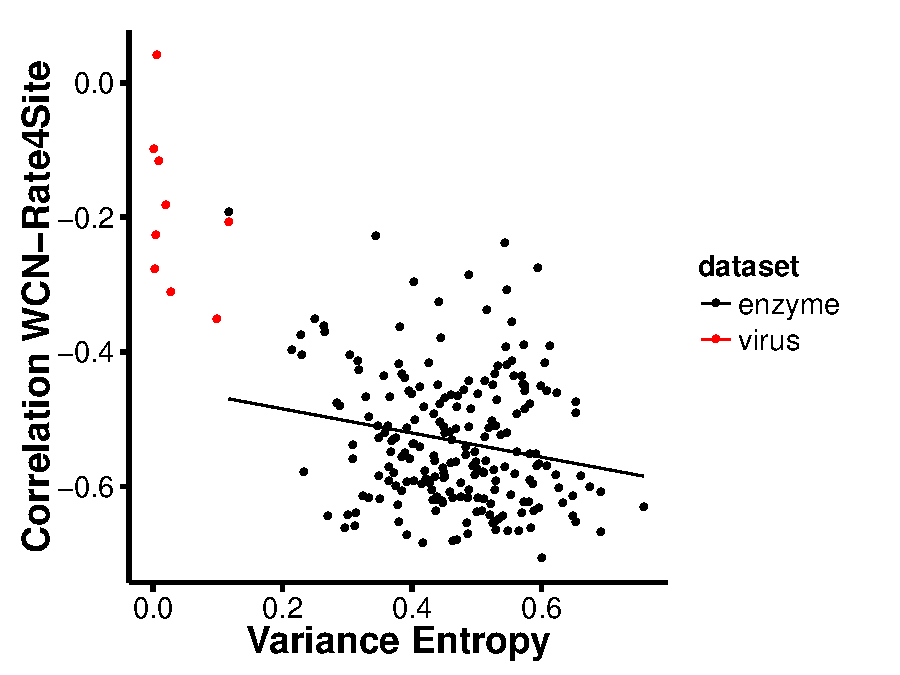
\includegraphics[width=5.0in]{var_entropy_rate_cor.pdf}}     
            \caption{NEED A CAPTION!!!.}
            \label{fig:seqent_structure_cors}
    \end{figure}
    
Figures that are still needed...
Table 1 - First make a new table with the mean values Entropy
Table 2 - First make a new table with the mean values Rate4Site

\begin{center}
	\begin{table}
	\begin{tabular}{| p{1.5cm} | p{2.5cm} | p{2cm} | p{2cm} | }
		\hline
		Dataset & Mean $\rho$ Entropy-CN  & Mean $\rho$ Entropy-WCN & Mean $\rho$ Entropy-RSA \\
		\hline	
		Enzyme &  $-0.445$  & $-0.432$ & $0.464$ \\
		\hline
		Virus & $-0.213$ & $-0.217$ & $0.237$ \\
		\hline	
	\end{tabular}
	\caption{NEED A CAPTION}
	\label{table:entropy_stats}
	\end{table}
\end{center}



\begin{center}
	\begin{table}
	\begin{tabular}{ | c | c | c | c |  }
	\hline
	Model & Coefficient x  & Coefficient y & Coefficient z \\	
	\hline
	Enzyme & $-0.562$ & $-0.533$  &  $0.548$ \\
	\hline
	Virus & $-0.172$ & $-0.192$ &  $0.190$ \\
	\hline
	\end{tabular}
	\caption{NEED A CAPTION}
	\label{table:rate_stats}
	\end{table}
\end{center}



Need a two panel figure \\
First plot the mean entropy vs the variance of entropy (then pick points that are in each of the four corners). This is B. I need to circle these by pointing an additional geom point and open circles and put numbers.  \\
Pick these proteins and then plot the distributions. This is A. \\
Basically this figure will highlight the difference between mean entropy and variance in entropy. \\ 

In the introduction and abstract need to better highlight the two papers (Yeh and Shah) that contradict on the surface and they do not. Hold off on Rate4Site for Now.

\end{document}

